\chapter[Análise dos Resultados Obtidos]{Análise dos Resultados Obtidos}
\label{ch:capfinal}

Neste capítulo, será apresentada a análise de resultados, relativos ao teste de usabilidade, orientando-se pela metodologia 
descrita na seção \ref{vsf}. Portanto, constam seções dedicadas: a formulação do problema; definição da unidade 
caso; determinação do número de casos; elaboração do protocolo; coleta de dados e avaliação e análise de dados.
Por fim, têm-se as considerações finais do capítulo

\section{Formulação do Problema}
O ciclo menstrual tem duas fases principais: a fase folicular e a fase lútea. Dessas, a fase folicular 
pode 
ser dividida em fase folicular inicial, na qual ocorre a menstruação, e a fase folicular final, na qual 
há a liberação do óvulo.
Quando o óvulo é liberado, tem início a fase lútea, que também pode ser dividida em fase lútea inicial e 
fase lútea final, sendo quando, para algumas pessoas, acontece a TPM.

Durante essas fases, as pessoas passam por várias mudanças hormonais, que podem influenciar nas tarefas 
cotidianas, demandando mais energia para a realização de certas tarefas. Na fase folicular final e lútea inicial, de acordo com a referência bibliográfica, 
foi relatada uma melhora significativa no desempenho das atividades cognitivas e verbais, enquanto no final da fase 
lútea, há a relação com o aumento do cortisol, hormônio do stress e uma certa dificuldade na classificação 
no reconhecimento de expressões, tendendo a reconhecer expressões neutras como negativas. Outros fatores como a TPM, que envolve
mudança de humor e comportamento, também são relatadas. Na menstruação, é comum que sintam sintomas físicos, como cólicas, demandem 
atividades físicas com menos esforço e prejudiquem a concentração. 

Tendo o conhecimento dessas influências, é proposto, então, um sistema de sugestão, utilizando os algoritmos de sistema de recomendação, 
que indicaria tarefas que seriam mais facilmente ou dificilmente realizadas dependendo do perfil e da fase do ciclo menstrual da pessoa.

Esse sistema poderá ajudar no autoconhecimento de quem o utiliza, melhorando a inteligência emocional e fazendo com que 
as mulheres possam utilizar dos benefícios e lidar com os malefícios de cada fase de forma saudável e consciente.

No escopo deste trabalho, foi possível montar um processo de contagem de ciclo para determinar em que fase a pessoa se encontra, utilizando o 
método do calendário.

Foi utilizado o estudo de caso para realizar a coleta de dados a análise de resultados, anteriormente descritos nas seções \ref{vsf1} e \ref{vsf2}, 
sobre o perfil das mulheres e para determinar quais tarefas iriam demandar 
menos ou mais energia para serem executadas, além disso, também foi possível estabelecer quatro grupos de recomendação iniciais, sendo que o 
primeiro é para mulheres que utilizam método contraceptivos hormonais, o segundo para mulheres que não utilizam métodos contraceptivos hormonais e 
não possuem distúrbios endócrinos, e o terceiro é para mulheres que não utilizam métodos contraceptivos hormonais e possuem distúrbios endócrinos. 
Um desses três grupos é atribuído a usuária quando ela cria uma conta e responde o questionário do aplicativo Mina. 

Os grupos foram inicialmente carregados com características das tarefas apontados pelos perfis descritos acima em um segundo questionário. 
O quarto grupo foi inicialmente carregado com informações inferidas pelo referencial teórico. 

Quando a usuária envia uma avaliação das tarefas, são realizados alguns cálculos através do método de contagem de inversões para determinar 
a qual grupo a usuária está realmente mais próxima, esses grupos são retro alimentados com as pontuações dadas pelas usuárias pertencentes a eles.

\section{Definição da Unidade Caso e Determinação do Número de Casos}

A unidade caso é do tipo estudo de caso coletivo. Esse tipo de estudo tem o propósito de estudar características
de uma população, no caso deste trabalho, mulheres, jovens, entre 20 e 35 anos, em idade fértil, cursando ou 
formadas em um curso de graduação. 

Essas mulheres, então, possuem alto grau de instrução e acesso a informação. Elas possuem um bom nível de conhecimento sobre o 
funcionamento do próprio corpo e tem acesso a diversos tipos de métodos contraceptivos. Algumas optaram por não utilizar 
métodos contraceptivos hormonais. 

Ao longo do estudo as mulheres foram instruídas para ficarem atentas as mudanças do próprio corpo, fazendo anotações pessoais 
da forma que acharem mais confortável.

Após o primeiro ciclo realizado na primeira parte desse trabalho, foi possível dar andamento no desenvolvimento da aplicação, 
que resultou no aplicativo Mina, disponibilizado apenas para aplicativos Android. Caracterizando o grupo do teste de usabilidade como 
usuárias Android.

O grupo, formado pela Autora, contava, inicialmente, com 23 mulheres, mais que o dobro do número considerado ideal 
para um estudo de caso (quatro a 10 pessoas). 
O primeiro ciclo contou com a participação de todas, mas por causa do tempo de realização entre a primeira e segunda parte desse trabalho, 
algumas mulheres acabaram saindo do grupo ou simplesmeste perdendo o interesse. Outra barreira foi o lançamento apenas para plataforma Android. 
Ao final, houve a participação efetiva de 7 mulheres que compunham desde o início esse grupo.


\section{Elaboração do Protocolo e Coleta de Dados}


O protocolo elaborado envolve: visão global do projeto, procedimentos de campo, determinação das questões e guia para a elaboração do relatório.
A visão global do projeto descreve o propósito e o cenário em que foi desenvolvido o estudo. Nesse caso, o propósito é o teste do aplicativo Mina, que contém 
um sistema de recomendação de tarefas baseadas 
em perfil e fase do ciclo menstrual das mulheres. O cenário em que foi desenvolvido o estudo foi descrito na seção anterior.

O procedimento de campo envolveu a seleção das usuárias desse grupo que utilizassem Android e ainda tivessem interesse em contrubuir, participando 
do teste de usabilidade do aplicativo.

O aplicativo foi disponibilizado para Android através da ferramenta TestFlight do Firebase. As mulheres interessadas receberam um convite, 
baixaram a aplicação e 7 
delas responderam o questionário. 

A determinação das questões levaram em consideração o product backlog, utilizado como uma 
forma de modelagem de acordo com a metodologia Scrum, 
um \emph{product backlog} foi construído utilizando um total de 
sete temas: conta, questionário, sobre a fase, previsão, perfil, 
calendário e documentação. As histórias de usuário podem ser 
encontradas no repositório do github\footnote{repositório github: https://github.com/Mikhaelle/mina-tcc.}.

\begin{itemize}
\item P01: Conta -> envolverá a parte de criar uma conta nova e entrar em uma conta já existente;
\item P02: Questionário -> envolverá a criação do questionário inicial do aplicativo e sua edição;
\item P03: Sobre a Fase -> envolverá a criação de textos informativos sobre a fase;
\item P04: Previsão -> envolverá a sugestão de tarefas que podem aparecer na respectiva fase do ciclo;
\item P05: Perfil -> envolverá a edição do perfil, como mudança de senha e configurações;
\item P06: Calendário -> envolverá a criação do calendário que mostrará o ciclo completo e as fases, e
\item P07: Documentação -> envolverá toda a atividade de documentação do aplicativo.

\end{itemize}

O questionário\footnote{terceiro questionário : https://forms.gle/j7eCWStZPbT4Ppy59} foi feito utilizando a plataforma Google Forms e foi respondido de forma anônima, para que as
participantes se sentissem mais confortáveis respondendo-o. Ao todo, o questionário contou com 22 perguntas, sendo 18 fechadas 
(Tabela \ref{tab15} e \ref{tab17}) e 
quatro abertas (Tabela \ref{tab16}). Foram recebidas 7 respostas até a data 13/04/2022. Todas as respostas estão 
detalhadas no relatório no Apêndice \ref{usertest} .

\begin{table}[ht]
    \centering
    \caption{Perguntas Abertas do Terceiro Questionário}
    \label{tab16}
    \begin{tabular}{c}
        \toprule
        \textbf{Perguntas abertas} \\
        \midrule     
        \begin{minipage} [t] {1\textwidth} 1 - (P01) Você teve alguma dificuldade com o processo de criação de conta e login? Teria alguma sugestão de melhoria?\end{minipage} \\
        \midrule
        \begin{minipage} [t] {1\textwidth} 2 - (P02) Você teve alguma dificuldade para responder o questionário? Teria alguma sugestão de melhoria?\end{minipage}\\
        \midrule
        \begin{minipage} [t] {1\textwidth} 3 - Você teve alguma dificuldade nos processos anteriores ?  \end{minipage}\\
        \midrule
        \begin{minipage} [t] {1\textwidth} 4 - Você teria alguma sugestão de melhoria para os processos anteriores? \end{minipage}\\
        \bottomrule
    \end{tabular} 
\end{table}

\begin{table}[ht]
    \centering
    \caption{Perguntas Fechadas do Terceiro Questionário - Parte 1}
    \label{tab15}
    \begin{tabular}{c}
        \toprule
        \textbf{Perguntas fechadas} \\
        \midrule
        \begin{minipage} [t] {1\textwidth} 1 - (P01) Tente criar uma conta utilizando email, nome de usuário e senha ao clicar em criar conta ou entrar utilizando uma conta do Google. Você conseguiu?
        \end{minipage} \\
        \midrule
        \begin{minipage} [t] {1\textwidth} 2 - (P01) Você teve alguma dificuldade com o processo de criação de conta e login? Teria alguma sugestão de melhoria?
        \end{minipage}\\
        \midrule
        \begin{minipage} [t] {1\textwidth} 3 - (P02) Ao entrar na conta a primeira vez é esperado que você tenha que responder um pequeno questionário em que a primeira tela é para selecionar a data da ultima menstruação. Essa tela apareceu? \end{minipage} \\
        \midrule
        \begin{minipage} [t] {1\textwidth} 4 - (P02) Tente responder todas as perguntas do questionário. Você conseguiu finalizar esse processo? \end{minipage}  \\
        \midrule
        \begin{minipage} [t] {1\textwidth} 5 - (P06) É esperado que a primeira tela que apareça após responder o questionário seja a do calendário. Essa tela apareceu? \end{minipage}\\
        \midrule
        \begin{minipage} [t] {1\textwidth} 6 - (P06) Você conseguiu identificar qual fase do ciclo você está? \end{minipage} \\
        \midrule
        \begin{minipage} [t] {1\textwidth} 7 - (P06) O calendário está coerente, começando na data da sua ultima menstruação e tendo o tamanho do ciclo respondido no questionário? \end{minipage}\\
        \midrule
        \begin{minipage} [t] {1\textwidth} 8 - (P04) Tente acessar a recomendação de tarefas na previsão de hoje. Pode ser que uma mensagem dizendo que as recomendações estão sendo geradas apareça. Essa mensagem apareceu para você? \end{minipage}\\
        \midrule
        \begin{minipage} [t] {1\textwidth} 9 - (P04) As recomendações levam de 1 a 5 min para aparecerem após a criação da conta, tente acessar novamente durante esse tempo. Aproveite para responder as outras questões enquanto as recomendações não aparecem. Quanto tempo demorou para as recomendações aparecerem? \end{minipage}\\
        \bottomrule
    \end{tabular}
\end{table}



\begin{table}[ht]
    \centering
    \caption{Perguntas Fechadas do Terceiro Questionário - Parte 2}
    \label{tab17}
    \begin{tabular}{c}
        \toprule
        \textbf{Perguntas fechadas} \\
        \midrule
        \begin{minipage} [t] {1\textwidth} 10 - (P03) Na página do calendário, entre em sobre a fase. Você achou util um texto explicativo sobre a fase? \end{minipage}\\
        \midrule
        \begin{minipage} [t] {1\textwidth} 11 - (P04) Tente acessar a aba avaliação pelo menu inferior. Uma lista com as tarefas e opções entre mais fácil, neutro e mais difícil apareceu? (É possível que as recomendações ainda não tenham sido geradas, espere um pouco) \end{minipage}\\
        \midrule
        \begin{minipage} [t] {1\textwidth} 12 - (P04) Selecione as opções correspondentes a tarefa e envie a avaliação. Uma mensagem dizendo que a avaliação foi enviada apareceu? \end{minipage}\\
        \midrule
        \begin{minipage} [t] {1\textwidth} 13 - (P04) Volte a aba de previsão de hoje. Você notou alguma mudança nas recomendações? \end{minipage}\\
        \midrule
        \begin{minipage} [t] {1\textwidth} 14 - (P05) Tente acessar o perfil pelo menu inferior e sair da aplicação, você foi redirecionado para o login ? \end{minipage}\\
        \midrule
        \begin{minipage} [t] {1\textwidth} 15 - (P01) Tente recuperar a senha em esqueci a senha inserindo o seu email. Você recebeu um email para recuperação de senha? \end{minipage}\\
        \midrule
        \begin{minipage} [t] {1\textwidth} 16 - (P01) Tente entrar novamente, agora com a conta ja criada você foi direcionado para a página inicial com o calendário? \end{minipage}\\
        \midrule
        \begin{minipage} [t] {1\textwidth} 17 - (P06) Por último, tente adicionar um novo ciclo. Você conseguiu? \end{minipage}\\
        \midrule
        \begin{minipage} [t] {1\textwidth} 18 - (P06) O calendário atualizou com os dados do novo ciclo? \end{minipage}\\
        \bottomrule
    \end{tabular}
\end{table}


\section{Avaliação e Análise dos Dados}



Um problema que surgiu na aplicação do teste foi a utilização do \emph{dark mode} no celulares de algumas usuárias. O \emph{dark mode} 
modifica as cores do aplicativo e como esse tipo não estava rastreado para ser utilizado no aplicativo, acabou gerando alguns \emph{bugs} 
como ícones desaparecendo. Assim que detectado o problema, foi proposto às usuárias que desabilitassem o \emph{dark mode} antes de realizar o teste.

\textbf{Resultados das perguntas correspondentes ao \emph{product backlog} P01 - Conta:} Features como, criação de conta, login, resete de 
senha e logout foram bem avaliados e nenhuma participante dos testes relatou problema nessa parte. 
Houve uma sugestão de adicionar um campo para confirmação de senha ao criar uma conta.


\textbf{Resultados das perguntas correspondentes ao \emph{product backlog} P02 - Questionário:} Em todos os casos, ao criar uma conta nova a pessoa tinha que responder o 
questionário e depois era direcionada a \emph{home}. A feature de questionário 
funcionou como esperado, apenas alguns problemas de ortografia foram relatados pelas usuárias. Houve uma sugestão para aumentar o 
número máximo do ciclo menstrual, aumentar a área dos botões com \emph{dropdown} que pode ser precionada e especificar se a 
data da menstruação requerida é do 
primeiro ou último dia da última menstruação.

\textbf{Resultados das perguntas correspondentes ao \emph{product backlog} P03 - Sobre a Fase:} Todas as usuárias acharam útil as informações 
sobre a fase. Houve uma sugestão de mudança de estilo da fonte do texto, pois a pessoa encontrou dificuldade na leitura.


\textbf{Resultados das perguntas correspondentes ao \emph{product backlog} P04 - Previsão:} Sobre a recomendação, houveram 
problemas de latência para que elas fossem geradas, uma usuária relatou que teve que esperar de um a três 
minutos para que elas aparececem, uma relatou entre um a três minutos, três relataram entre três a cinco minutos, uma 
relatou entre cino a sete minutos e uma mais que sete minutos. Foi identificado que o problema de latência é 
decorrente da localização diferente do servidor do banco de dados (\emph{southamerica-east1}) e as 
funções do Cloud Functions (\emph{us-central1}). Também foi relatado 
uma dificuldade em entender o significado das setas ou traços na página de recomendação. Foi sugerido 
então um tutorial inicial no aplicativo ou a inserção de uma legenda sobre os significados.

Na tela de avaliação nenhuma usuária relatou dificuldade em avaliar as tarefas. Houve um problema relatado 
em celulares menores em que a opção 'mais fácil' ficava cortada, apesar disso ainda continuou possível selecionar 
essa opção. As avaliações foram enviadas corretamente.

\textbf{Resultados das perguntas correspondentes ao \emph{product backlog} P05 - Perfil:} As usuárias conseguiram acessar o perfil 
e visualizar seus nomes, o botão de refazer o questionário e o de sair. Essa feature não foi totalmente implementada, pois faltou a 
parte de redefinição de senha elicitado nos requisitos.

\textbf{Resultados das perguntas correspondentes ao \emph{product backlog} P06 - Calendário:} As usuárias não tiveram problemas 
para identificar qual fase do ciclo elas estavam e o calendário estava coerente com os dados setados no questionário inicial.
Houve uma sugestão para adicionar uma legenda para as cores das bolinhas nos questionário e quais são as fases correspondentes. 

Uma participante do teste foi auxiliada através de uma entrevista guiada pelo 
questionário para que fosse possível captar as mudanças dos grupos em tempo real. 

Ao responder o questionário a primeira vez, a usuária foi inserida no grupo 3 (Vide Figura \ref{fig23}), 
após enviar a avaliação, os pontos foram somados 
na tabela do usuário e o grupo dela foi atualizado para o grupo 2 (Vide Figura \ref{fig24}) 
que foi dado como mais próximo pelas contagens de inversão. 
Os pontos do usuário então foram inseridos no grupo 2 (Vide Figura \ref{fig25}). O uid dos usuários foi apagado nas 
imagens por questões de segurança.

Após as usuárias criarem as contas, responderem os questionários e enviarem os feedbacks, foi possível observar que algumas 
mudaram de grupo e que as pontuações para as tarefas das usuárias e dos grupos foram atualizadas corretamente, demonstrando que 
a função de \emph{feedback} teve o comportamento esperado. 

\begin{figure}[ht]
	\caption{Grupo e Tarefas da Usuária Antes da Avaliação}
	\begin{center}
	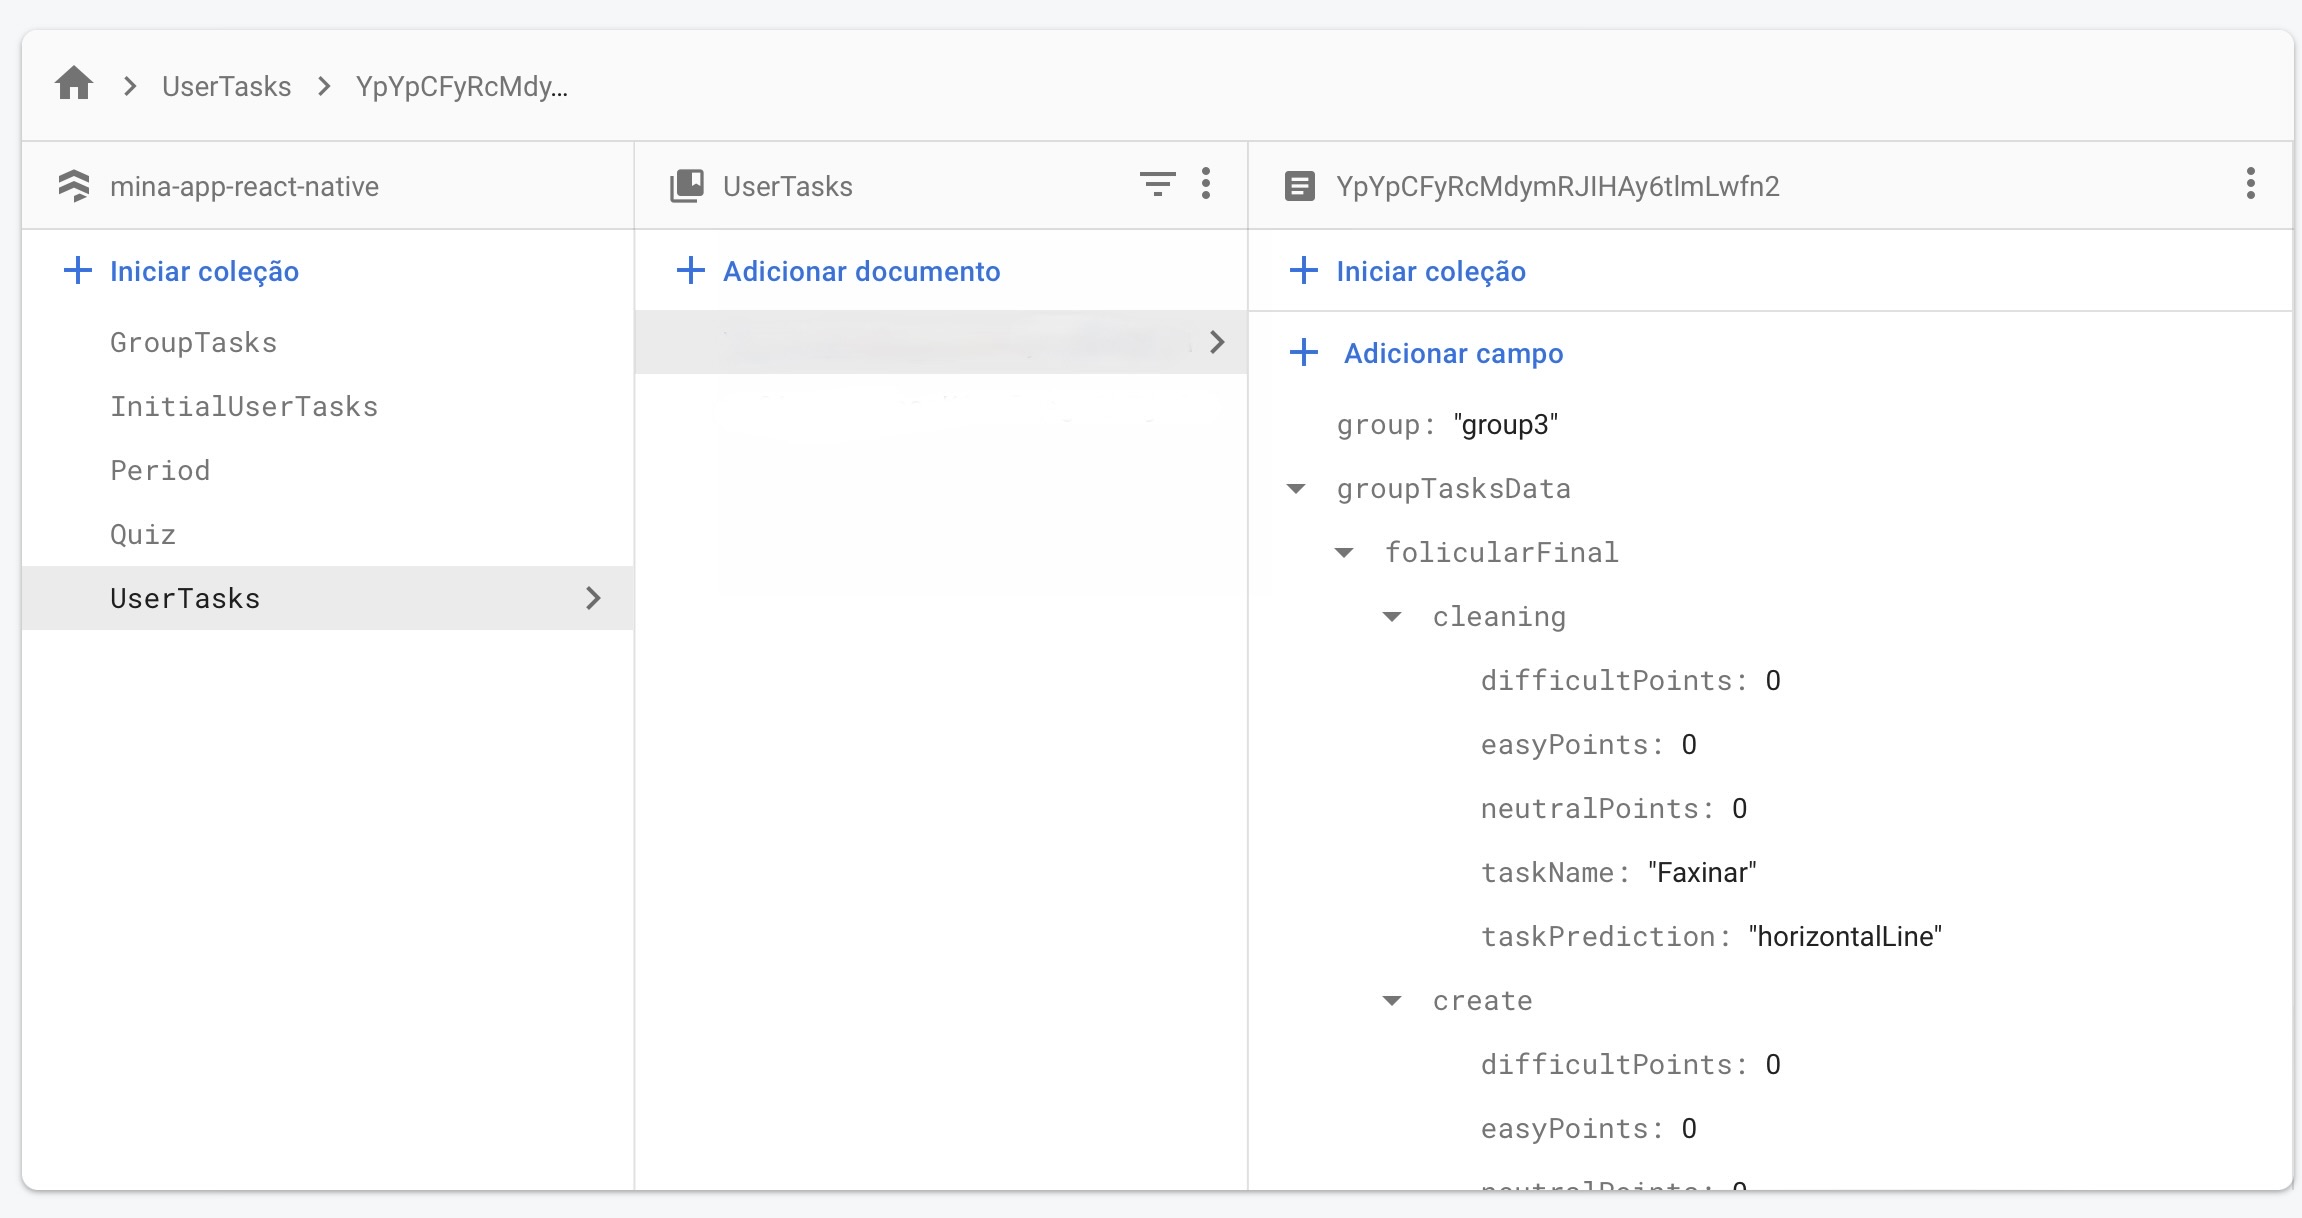
\includegraphics[keepaspectratio=true,scale=0.18]{figuras/db1.jpeg}
	\end{center}
	\legend{Fonte: Autora}
    \label{fig23}
\end{figure}

\begin{figure}[ht]
	\caption{Grupo e Tarefas da Usuária Depois da Avaliação}
	\begin{center}
	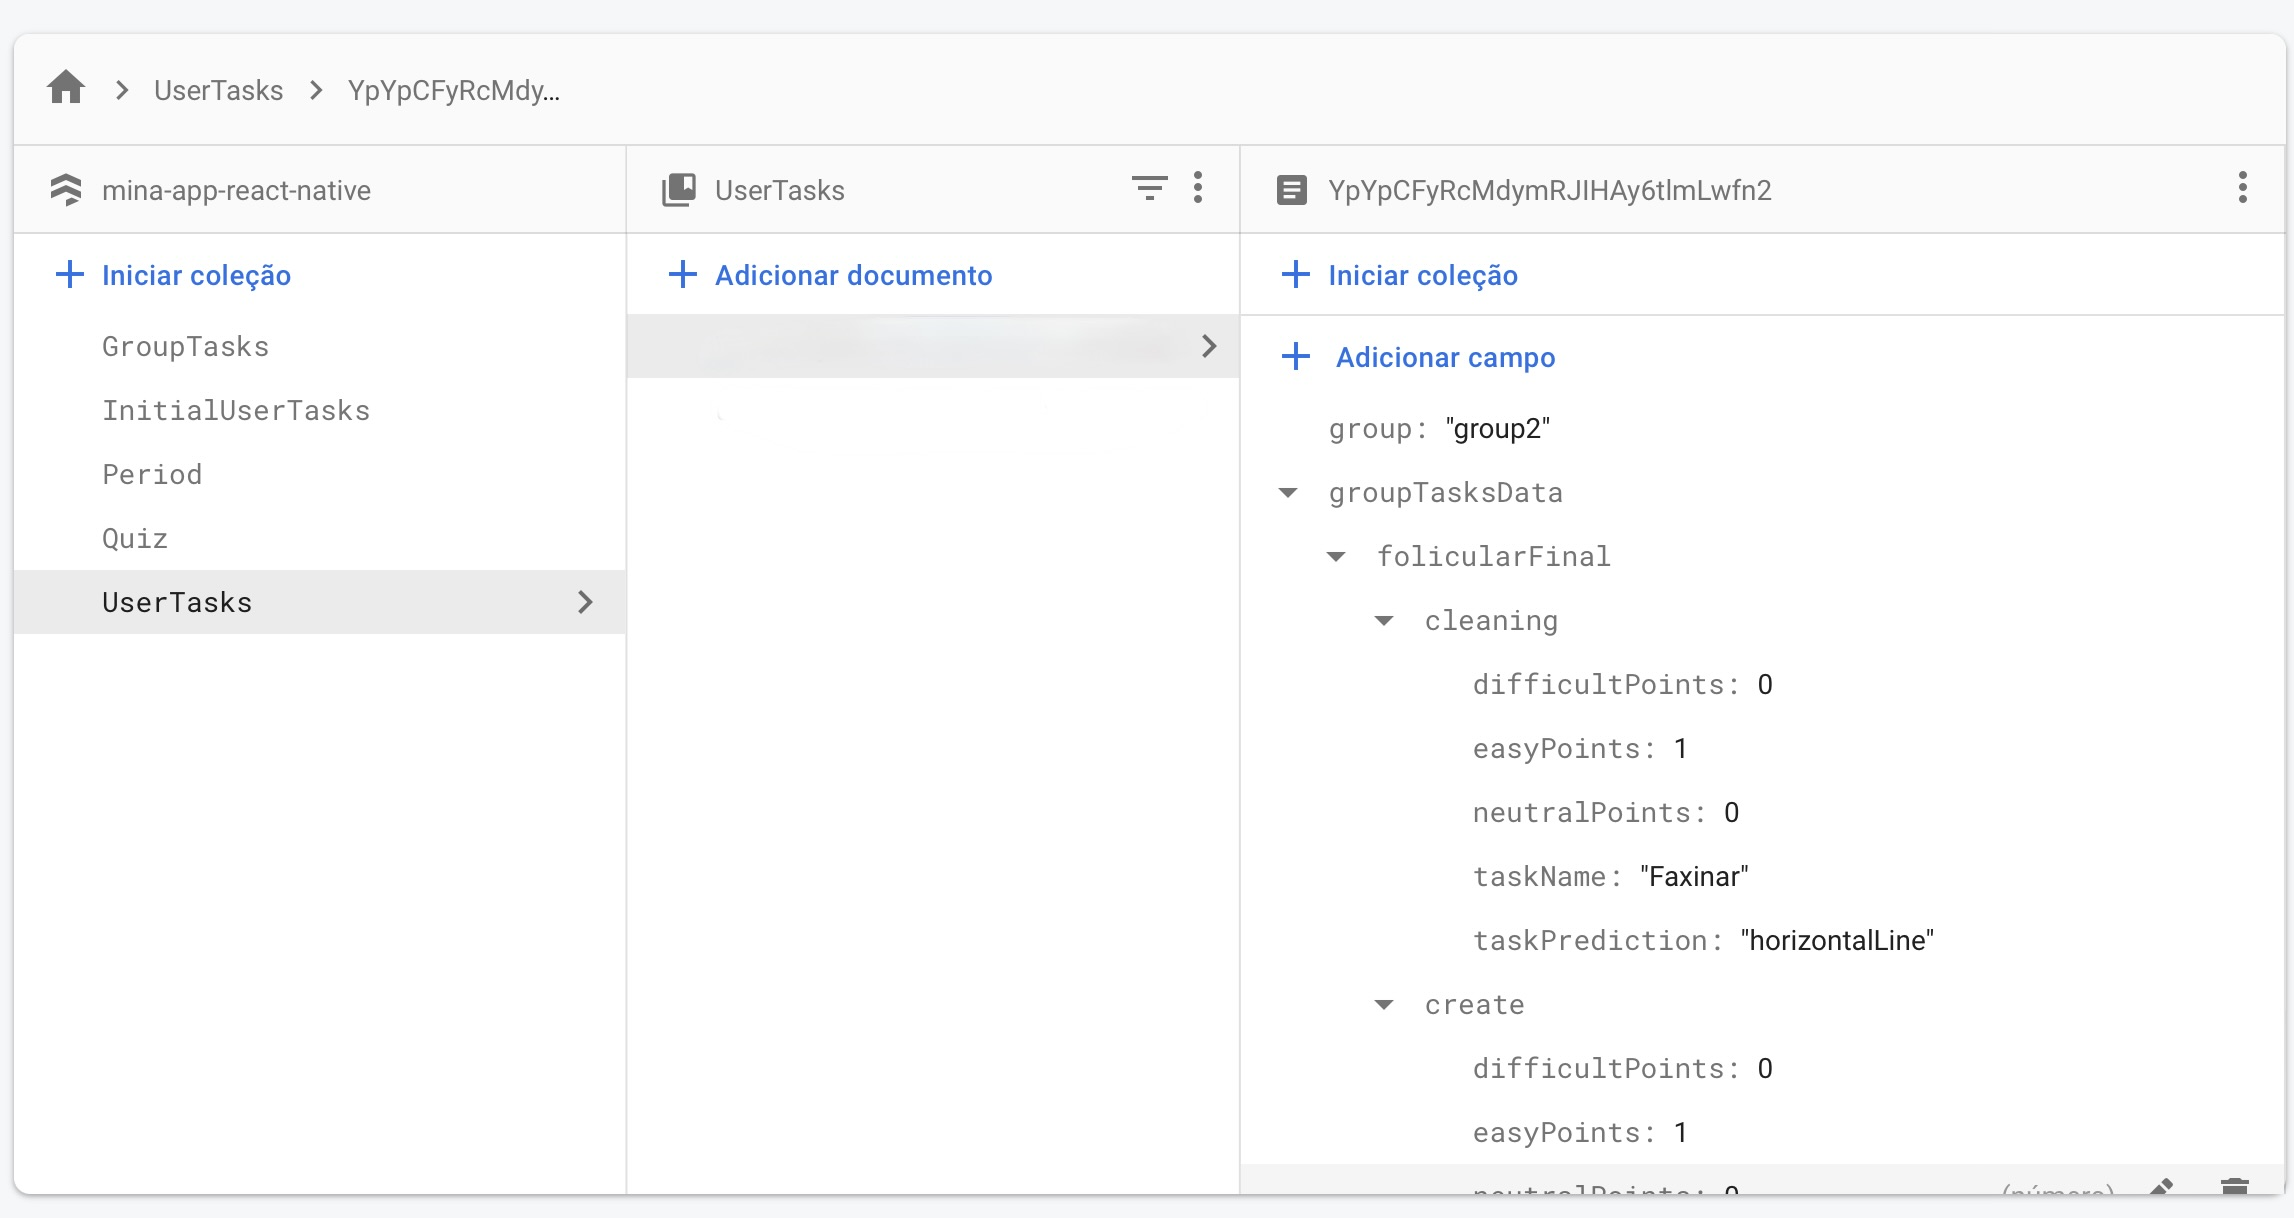
\includegraphics[keepaspectratio=true,scale=0.37]{figuras/db4.jpeg}
	\end{center}
	\legend{Fonte: Autora}
    \label{fig24}
\end{figure}

\begin{figure}[ht]
	\caption{Grupo com Pontuações da Usuária Adicionados}
	\begin{center}
	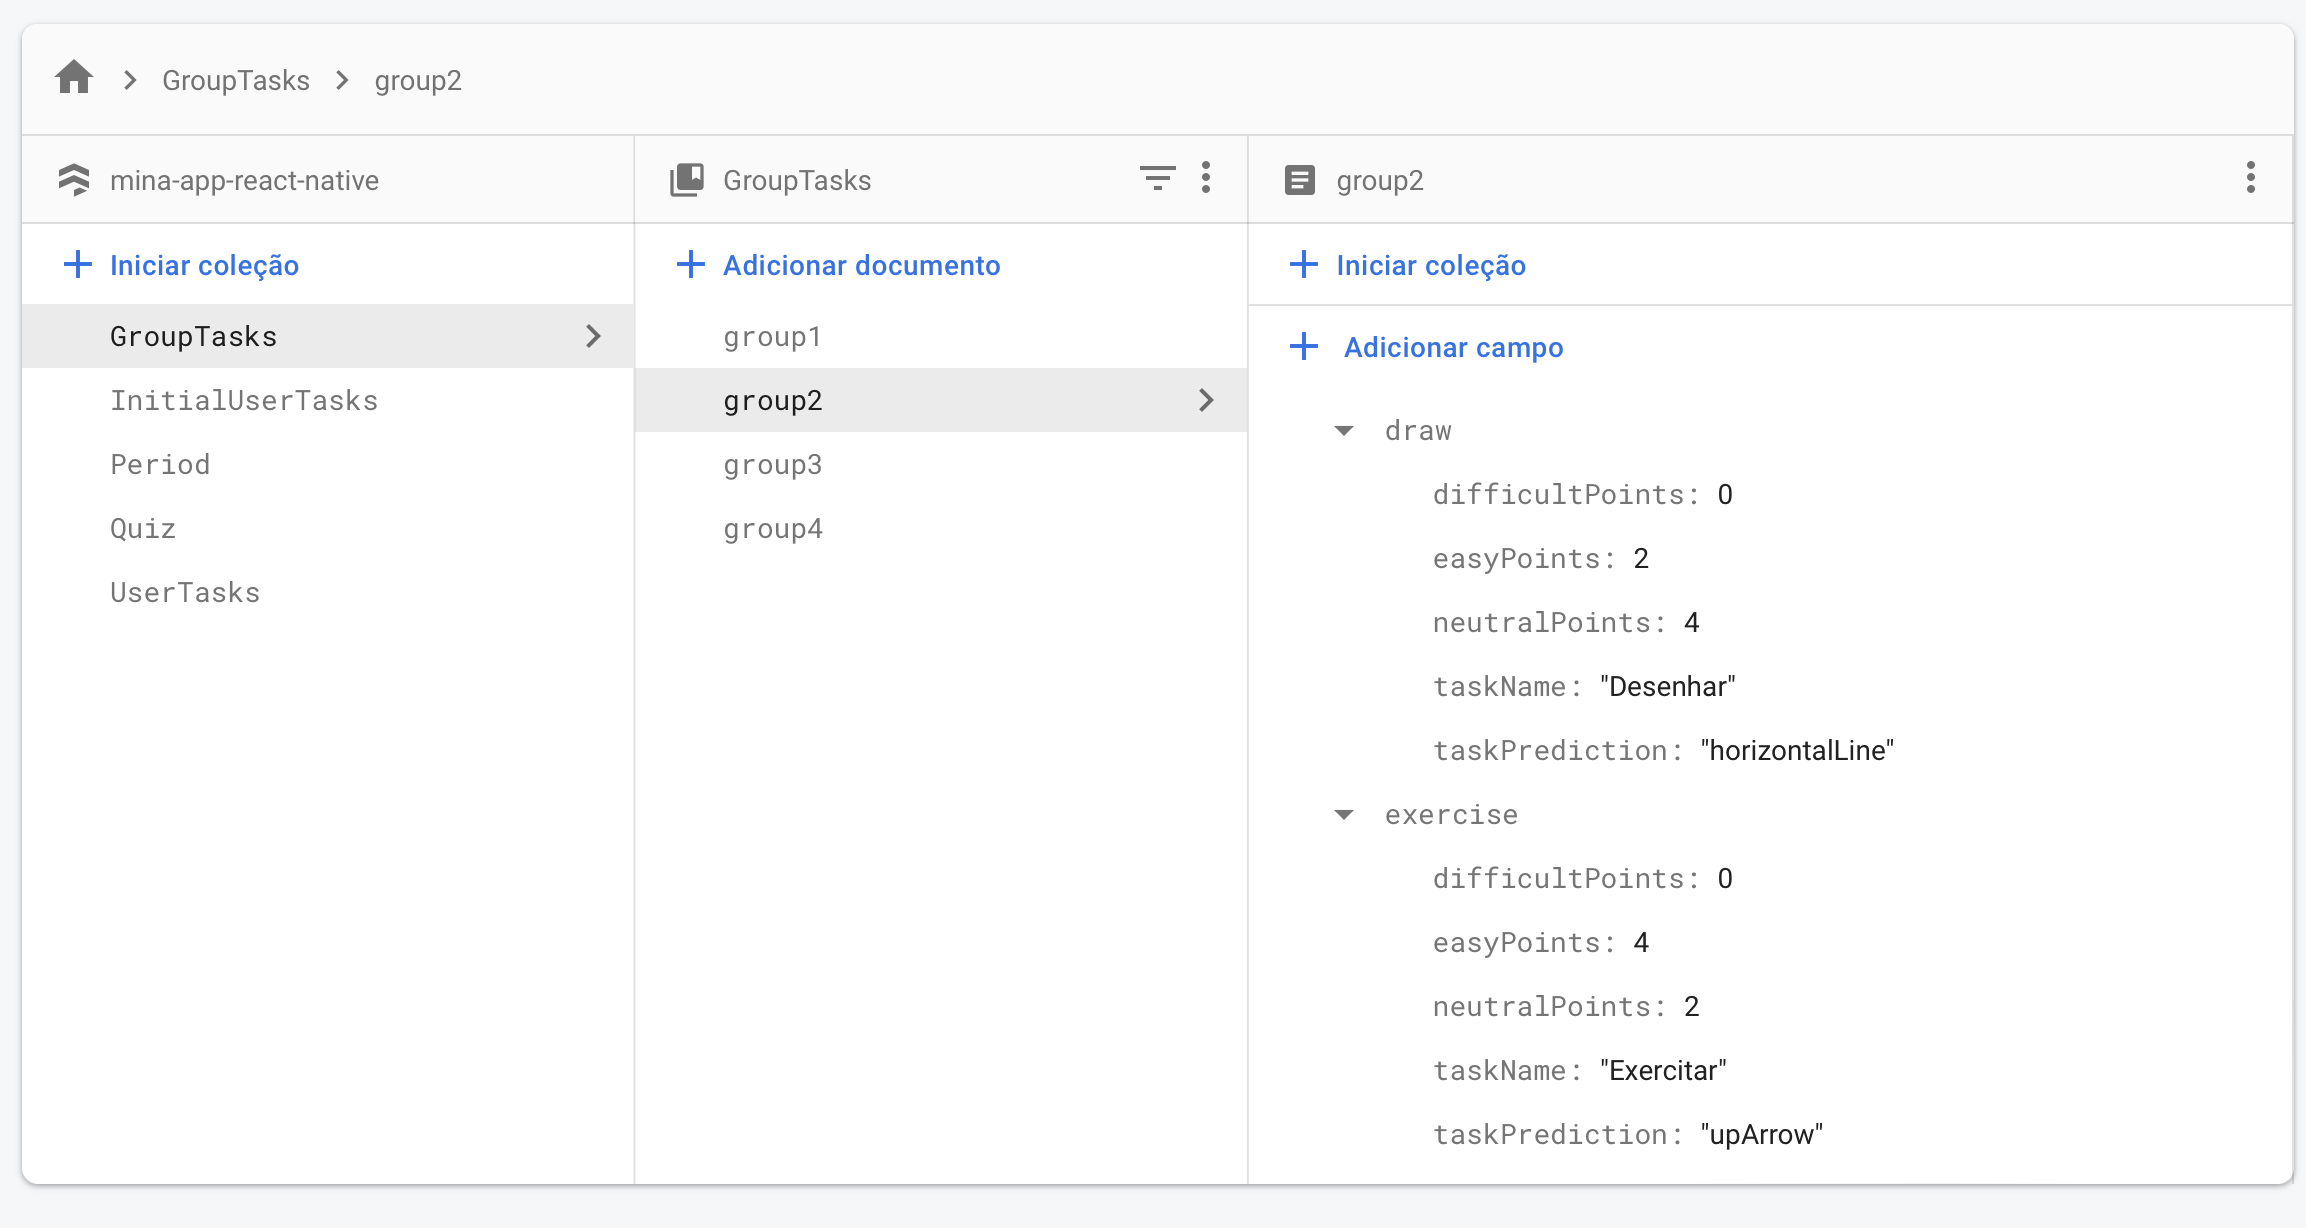
\includegraphics[keepaspectratio=true,scale=0.37]{figuras/db3.png}
	\end{center}
	\legend{Fonte: Autora}
    \label{fig25}
\end{figure}


\section{Considerações Finais do Capítulo}

Ao longo do TCC1, foi possível vivenciar algumas atividades relevantes, tais como:

\begin{itemize}
    \item pesquisa e escrita científica;
    \item fechamento de escopo do trabalho;
    \item embasamento teórico e tecnológico;
    \item detalhamento metodológico;
    \item apresentação da proposta, das principais contribuições pretendidas com a realização da mesma e da prova de conceito, e
    \item acompanhamento contínuo das realizações, com reuniões periódicas entre orientado e orientador.
\end{itemize}

Ao longo do TCC2, foi possível vivenciar algumas atividades relevantes, tais como:

\begin{itemize}
    \item realizar correções da banca;
    \item desenvolvimento do aplicativo;
    \item aplicar metodologia estabelecida;
    \item realização do teste de usabilidade;
    \item documentação de melhorias e
    \item acompanhamento contínuo das realizações, com reuniões periódicas entre orientado e orientador.
\end{itemize}

Neste capítulo, foram apresentados os resultados obtidos com o estudo de casos aplicado a um grupo formado pela autora que conta com 
mulheres em idade fértil. Os resultados encontrados
estão vinculados aos objetivos gerais e específicos estabelecidos para esse trabalho. No próximo capítulo,
esses objetivos e outros aspectos serão retomados e debatidos com base nos resultados
obtidos e apresentados nesse capítulo.